\chapter{绪\hskip 0.4cm 论}
\label{ch1}

\section{研究背景及意义}
在过去的近十年,人工智能(Artificial Intelligence,AI)取得了令人难以置信的进步,机器学习也越来越广泛地应用于各种领域,包括医疗健康、自动驾驶、金融贸易等。为了进一步提高模型的训练精度和学习能力,新兴的深度神经网络,也称为深度学习(Deep Learning,DL)随之提出。深度学习算法的目标是通过从数据中泛化来学习如何执行某些任务,比如说图像分类、语音识别、自然语言翻译等。深度学习作为最有前景的技术之一,已广泛应用于图像分类、自动驾驶、智慧医疗等各个方面。例如,智能图像识别系统已广泛部署在机场、火车站等公共场所。 在识别可疑恐怖分子和检测违禁物品方面,它已被证明比人类更精确。基于基于患者的医疗数据,基于深度学习的回归技术可以帮助诊断和预防某些疾病(例如,遗传性和传染病)。很明显,基于深度学习的服务正在从旅行、社交、经济等诸多方面慢慢改变我们的生活。

深度学习算法的输入数据通常表示为一组样本。每个样本将包含一组特征值。例如,考虑一张 100x100 像素的照片,其中每个像素由一个数字(0-255 灰度)表示。我们可以用这些像素值组成一个长度为 10,000 的向量,通常称为特征向量。每张照片,表示为一个特征向量,可以与一个标签(例如,照片中人物的名字)相关联。深度学习算法将使用由多个特征向量及其相关标签组成的训练集来构建深度学习模型,这个过程称为模型的训练。当呈现一个新的测试样本时,深度学习模型应该给出预测的标签。模型准确预测标签的能力是衡量该模型对未知的数据的泛化程度的标准。它是通过测试误差(泛化误差)凭经验衡量的,它可以取决于用于训练模型的数据的质量和数量、使用什么深度学习算法来构建模型、深度学习算法超参数的选择(例如使用交叉验证),甚至是特征的提取方法。

一般来说,训练数据量在某种程度上决定了模型的性能。为了支持基于机器学习/深度学习的开发不断增长的需求,许多互联网云提供商推动机器学习即服务(DLaaS),为机器学习/深度学习模型训练和服务提供计算平台和学习框架。典型的机器学习即服务平台包括 Amazon Sagemaker、Google Cloud ML Engine、Microsoft Azure ML Studio。要使用MLaaS,客户需要向云提供商提供训练数据集和机器学习/深度学习算法。云提供商搭建深度学习环境,分配一定的计算资源,自动运行模型训练任务。云提供商还可以提供模型服务,将在云侧或客户侧训练的模型存储在云平台中。最后,云提供商向用户发布查询的API接口,使他们能够使用模型进行预测或分类。

训练数据集是训练和生成机器学习模型所必需的。数据集可能包含敏感样本,例如个人医疗记录、员工信息、财务数据等。我们的搜索查询、浏览历史、购买交易、我们观看的视频以及我们的电影的偏好都有可能被收集在使用的移动设备和计算机中。在街道上,以及即使在我们自己的办公室和家里。这种私人数据被用于各种深度学习应用。一些深度学习应用程序需要私人数据,此类私人数据以明文形式上传到集中的服务器,供深度学习算法学习数据中的规律,并从中构建模型。在2018年,中国互联网协会收到用户举报发现,腾讯音乐等多家应用软件以“通过深度学习向用户提供更好的服务”为由,长期收集并保存大量的用户个人数据,如照片、地址、电话等,甚至将这些包含了用户大量个人隐私的数据用作其他途径。问题不仅限于与将所有这些私人数据暴露在这些公司的内部威胁中,或外部威胁,如果持有这些数据集的公司遭到黑客攻击,那将会导致千万甚至亿万级的用户数据泄漏。

如何保护这些样本的隐私已成为机器学习中一个新的安全问题。这种隐私威胁在机器学习即服务中尤为严重。首先,在模型训练服务中,客户需要将训练数据上传到云提供商,提供商拥有数据的完全访问权限。过去的工作表明,恶意提供者可以轻松窃取敏感数据,将它们嵌入模型中实现隐私的泄漏。其次,在模型训练服务中,客户需要将预训练好的模型上传到云提供商,并设置端点供远程用户使用模型。成功的深度学习模型包含有关训练集的基本信息。因此,即使恶意提供者无法直接访问数据集,他也可以从模型参数中提取有关训练数据的敏感信息。第三,即使云提供商是可信的,只有黑盒访问模型输出结果的恶意远程用户仍然能够通过使用精心设计的输入查询模型来检索有关训练数据的信息。

针对这些问题,Google在2016年提出了联邦学习(Federated Learning,FL)的概念,它是一种典型的有助于解决多方计算下的隐私问题的学习方法。如图\ref{fig:联邦学习模型概况}所示,联邦学习的基本框架包含多个本地设备和一个中央服务器,所有训练数据保存在本地设备,所有设备共同协作训练一个全局模型。联邦学习实现了数据存储和模型训练的需求分离,使所有本地设备可以在不共享训练数据的情况下参与全局模型的训练。由于这种性质,联邦深度学 习受到了工业界和学术界的广泛关注,并且已经提出了各种分布式学习架构[3]、[4]、[5]来服务于特定场景。

\begin{figure}[!hbt]
\centering
	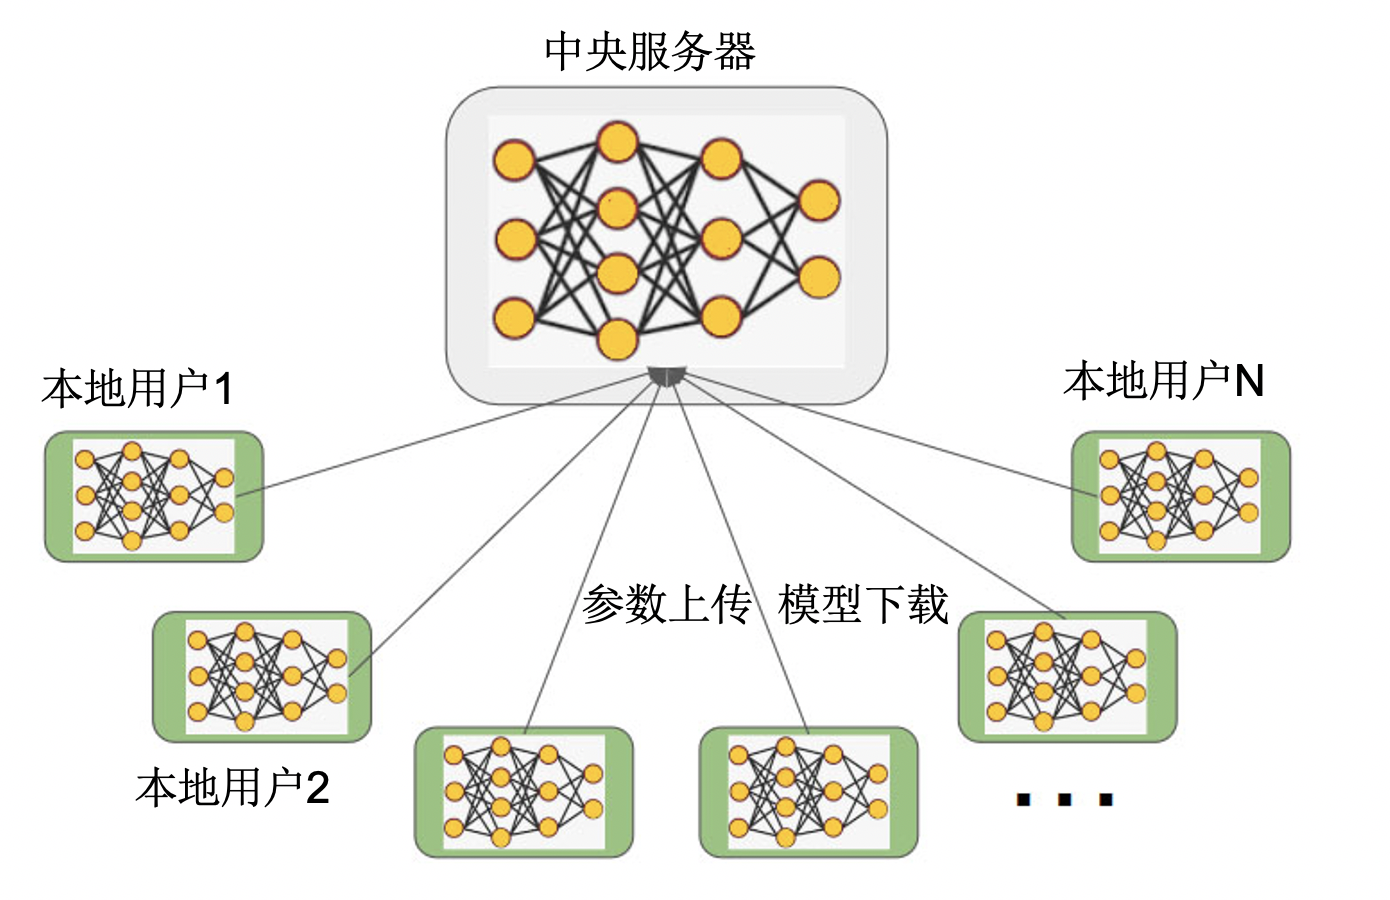
\includegraphics[scale=0.5]{fig2/C1/联邦学习}%联邦学习的系统架构
	\caption{联邦学习模型概况}
	\label{fig:联邦学习模型概况}	
\end{figure}

联邦学习允许更智能的模型、更低的延迟和更低的功耗。在联邦学习框架中,由于数据通常分布和存储在不同的位置(例如,数据中心和医院),无需集中联合学习使手机能够协作学习共享的预测模型,同时将所有训练数据保存在设备上,将深度学习的能力与数据存储在云中的需求分离开来,使用户可以在不共享本地数据的情况下在本地设备上进行预测。

\section{安全性和隐私威胁}
联邦学习的一个突出优点是它可以在服务器和客户端之间无需任何个人数据交换的情况下进行本地训练,从而防止客户端的数据被隐藏的对手窃听。尽管联邦学习的优势明显,而且与时俱进,但在实际应用之前,还需要对其安全性进行测试。近年来,大量的研究结果表明,联邦学习机制仍然存在安全问题,在训练过程中,本地设备与中央服务器之间的通信信道和传递的模型参数都有可能成为第三方窃取敏感信息的途径,联邦学习的框架仍然存在本地训练数据泄漏等隐私威胁。作为一种新的神经网络训练模型,攻击者可以从共享梯度中跟踪和获取参与者的隐私,联邦学习仍然面临各种安全和隐私威胁。

在联邦学习系统中,攻击方可能是内部攻击者,比如中央服务器、本地客户端;也有可能是外部攻击者。他们试图影响、破坏联邦学习模型的准确性,通过客户端上传的参数恶意的窃取用户的训练数据。

有一些恶意参与者会发送无效的模型参数更新到中央服务器,破坏全局模型的训练。比如,这些恶意参与方作为本地客户端参加训练,修改本地的训练数据,对本地数据注入一些有毒的数据,进行投毒攻击,从而损害全局模型的准确性,操纵模型的预测结果。

外部攻击主要通过本地客户端与中央服务器之间的通信信道发起。在训练过程中,局部模型更新和全局模型参数的结合过程,提供了关于训练数据的隐藏知识,用户的个人信息很有可能泄露给不受信任的服务器或其他恶意第三方。例如,白盒推理攻击和黑盒推理攻击\upcite{ref21}通过客户端上传的参数恶意的窃取用户的训练数据来生成样本原型。针对联邦学习中用户本地训练数据的攻击方式包括投毒攻击、模型重建攻击、模型反演攻击、成员推理攻击等。

投毒攻击:在联邦学习中,本地客户端在各自的设备上进行模型训练,将得到的训练参数上传给中央服务器。因为训练参数不需要通过可信机构的检查,所以有一些攻击者将恶意的训练样本注入自己的本地模型中,影响全局模型的更新结果,导致最终的模型预测结果错误甚至全局模型不可用。投毒攻击的影响对于许多企业和行业来说可能是致命的,在医疗部门、航空部门或道路安全方面甚至会危及生命。Marcus Comiter\upcite{ref56}曾使用投毒攻击进行实验,通过对熊猫的图像样本注入微小的恶意数据,导致算法预测结果发生重大变化,将熊猫识别为长臂猿。

模型重建攻击:在这种情况下,敌手的目标是窃取用户的原始训练数据。模型重建攻击需要白盒访问模型的权限,即模型中的特征向量对于敌手必须是已知的,敌手通过对特征向量的知识来重建用户的原始训练数据。对于一些机器学习算法,比如支持向量机(Support Vector Machine,SVM)或K最近邻算法(K-Nearest Neighbors,KNN),它们将特征向量存储在模型本身,容易受到重建攻击。攻击者通过解码用户上传的参数更新,反推出用户本地训练集中某条目标数据和其属性值。

模型反演攻击\upcite{ref11}:利用用户上传的参数信息,以一种很简单的方式攻击用户数据,一旦用户的网络模型经过训练并达到收敛,攻击者就可以通过调整网络模型权重的梯度, 获得网络模型中所有表示类的逆向工程试例。在模型反演攻击中, 攻击者无需接触目标信息的标签类,攻击模型仍然能够恢复原始样本试例。这一攻击模型表明,任何经过精确训练的深度学习网络,无论是以何种方式进行训练收敛, 都可以透露深度网络中不同标签类的信息。但是参数中包含的信息有限,模型反演攻击方式很难攻击卷积神经网络等复杂深度网络模型,在模型上添加了一定的隐私保护措施后,攻击也基本失效。

成员推理攻击\upcite{ref13}:给定一个深度学习模型和一条数据样本(敌手的知识),成员推理攻击旨在确定样本是否为用于构建此深度学习模型的训练集成员(对手的目标)。这种攻击可能是被对手用来了解某个人的记录是否用于训练深度学习模型,此类攻击利用深度学习模型对训练集中使用的样本与未包含的样本的预测差异。 Shokri 等人采用样本正确标签和目标模型预测的结果作为输入,训练影子模型作为攻击模型,达到推断任意样本是否在训练集中的目的。

\section{国内外研究现状}
随着针对联邦学习框架的攻击模型增多,研究人员开始关注训练联邦学习模型时存在的隐私安全问题。关于联邦学习的隐私定义主要分为全局隐私和局部隐私。在本地局部隐私中,每个客户端发送一个不同的隐私值,该值被安全的加密的上传到中央服务器。在全局隐私中,服务器在最终输出中添加不同的噪音以实现隐私保护。安全多方计算、同态加密\upcite{ref10}和差分隐私\upcite{ref9}是最常见的保证联邦学习中的安全和隐私的技术。

安全多方计算(Secure Multi-Party Computation,SMC)是由姚期智在1982年提出的\upcite{ref16},多个参与者在不泄露各自隐私数据情况下,利用隐私数据参与安全计算,共同完成某项计算任务。安全多方计算是解决协同计算问题的一种解决方案,它必须保证计算中各方信息的保密性、独立性和准确性。SMC安全模型自然涉及多方,各方除了自己的输入和输出一无所知,以确保完整的零知识安全证明。当前,安全多方计算领域常见的技术主要包括混淆电路、零知识证明、不经意传输和秘密共享等。

同态加密是一种加密形式,它允许用户对其加密数据执行计算,这些结果计算以加密形式保留,解密后的输出与未加密时进行相同计算操作产生的结果相同。同态加密可以分为加法同态加密、乘法同态加密和全同态加密。同态加密在联邦学习中的应用主要通过防止服务器对本地客户端上传的权重进行逆向工程从而反推出训练数据,确保每个客户端对全局模型的更改都保持隐藏状态。因为服务端接收的是本地客户端通过同态加密算法处理后的数据,这种模型的安全性是以服务器上的计算成本为代价的\upcite{ref23},这种加密场景的高计算复杂度会严重危害分布式机器学习设置的性能。

差分隐私(Differential Privacy,DP)方法的主要原理是向数据添加噪音,或使用概括方法来掩盖某些敏感属性\upcite{ref14},使至多相差1条数据的2个数据集的查询结果概率不可区分,以保护用户的隐私。在联邦学习框架中,通过在本地模型和全局模型中对相关训练参数添加噪声,进行扰动,使敌手无法获得真实的模型参数,进而防御模型反演攻击、成员推理攻击等。在深度学习中,差分隐私可以作为一种局部隐私保护方案来保护用户梯度的隐私,Ding M等人\upcite{ref24}提出了一种隐私保护的深度学习方法,主要通过添加噪声来扰乱本地模型的局部梯度,将差分隐私机制与模型训练中的随机梯度下降算法(Stochastic Gradient Descent,SGD)相结合。令人担忧的是,现有的差分隐私保护方案很难权衡隐私保护预算的成本和联邦学习模型的准确性,当使用较低的隐私预算达到较强的隐私保护的效果,可能使得模型难以收敛,可用性大幅下降;当隐私保护强度太低时,可能无法防御诸如GAN攻击等大规模的生成对抗网络攻击。

总的来说,安全多方计算基于复杂的计算协议,同态加密的运算成本非常高,而差分隐私破坏了数据的可用性,很难在模型性能和隐私成本上达到平衡,当前的研究方向主要集中在对数据集和神经网络中的参数的加密和隐私保护机制上,较少关注到模型整体框架等过程。目前的联邦学习中的隐私保护方法还有许多不足,不能在隐私性和模型可用性上都达到一个相对满意的效果,此外, 大部分方法是基于统一的、固定的参数设置,会导致模型迭代过程中累积大量隐私损失,使模型性能大幅下降。因此,在联邦学习场景下,保护用户隐私的同时维持模型准确性仍需大量的研究。

\section{本文工作与主要贡献}
针对联邦学习中隐私性和模型精度的双重指标,本文提出了本地自适应差分隐私算法和安全混洗框架,主要的工作和贡献包含以下三个方面:
\begin{enumerate}
\item [(1)] 在联邦学习差分隐私的场景下,本文提出了一种新型的、基于本地差分隐私的权重分配自适应干扰算法。在客户端本地训练的神经网络模型中,通过分析前向传播算法,计算每个属性类对于模型输出的贡献比,然后,我们设计了一个自适应噪声添加的方案,根据贡献率注入不同隐私预算的噪声。之后我们设计了动量组合机制分析加噪累积产生的隐私预算,并证明了算法满足$\left(\epsilon_{c}+\epsilon_{l}\right)$-差分隐私。与传统的注入噪声的方法相比,我们在相同的隐私保护程度下大大减少了噪声对模型输出结果的影响,提高了模型的准确性。
\item [(2)] 考虑到联邦学习中参数聚合器的攻击和针对参数传播信道的攻击,本文提出了一种新的安全聚合机制,在本地客户端和中心服务器之间新增混洗器,在用户将参数上传到云服务器之前,先对参数进行混洗,模型参数的更新被匿名的发送到混洗器,通过对模型参数的拆分和混洗实现客户端匿名,并且证明了安全混洗模型的可行性。
\item [(3)] 本文在三种数据集上进行实验,并与前人的方案进行对比,证明了自适应本地差分隐私方案和安全混洗框架的结合,在较低的隐私预算下还能使联邦学习模型维持较高的精度。
\end{enumerate}

\section{本文组织结构}

本文一共六章,主要内容的组织安排如下:

第一章对本文研究内容:联邦学习的研究背景、国内外研究现状进行了阐述,介绍了目前联邦学习中的攻击模型和隐私保护的研究现状和发展方向。

第二章详细介绍本文研究内容所涉及的一些理论基础与背景知识,包含了联邦学习的相关概念,差分隐私的基础知识和神经网络的基本结构。

第三章描述了本文所提出的本地自适应差分隐私算法的设计和实现,根据神经网络前向传播算法,分析属性值的贡献度,根据属性值添加自适应的拉普拉斯噪声,然后采用动量组合机制分析添加的噪声大小,并证明了在自适应差分隐私机制下的联邦学习算法的隐私性。
  
第四章在上一章的基础之上,提出了一种联邦学习安全混洗模型,混洗器对客户端上传的梯度进行采样后,然后拆分混洗,再将混洗模型和自适应本地差分隐私保护方法结合在联邦学习系统中,提高系统学习效果,最后证明了安全混洗模型的隐私性和收敛性。
    
第五章为实验部分,基于本文提出的隐私保护框架,我们在三个基准数据集的进行了实验和讨论,并与之前的差分隐私联邦学习框架进行对比实验。

第六章是对文本的工作内容的总结和未来研究方向的展望。首先对本文的研究内容进行了概括,并总结了现有方案的不足之处,之后对未来的研究和改进方向进行了展望。

\section{本章小结}
这一章节为绪论,首先介绍了本文章的研究背景和意义,总结了当前联邦学习发展过程中的挑战和难点,并具体针对联邦学习中的隐私威胁和隐私保护的研究现状做了具体的阐述,最后介绍了文章的主要研究、贡献和组织结构。

